\begin{enumerate}[label=\thesection.\arabic*.,ref=\thesection.\theenumi]
\numberwithin{equation}{enumi}
\item
Sketch the Polar Plot for
\begin{align}
G(s) = \frac{1}{(1+s)(1+2s)}
\end{align}
\\
\solution  Then the given open loop Transfer Function is
\begin{align}
G(s) = \frac{1}{(1+s)(1+2s)}
\end{align}

Now we have to substitute s=j$\omega$\\
\begin{align}
G(j\omega) = \frac{1}{(1+j\omega)(1+2j\omega)} 
\end{align}
\item
Then find the Magnitude of the Transfer Function
\\
\solution
\begin{multline}
      |G(j\omega)| = \frac{1}{\sqrt{(1+(\omega^2))(1+(2\omega)^2}}
\end{multline}\\
\item
Next find the Phase of Transfer Function\\
\solution
\begin{align}
    \angle G(j\omega) = \angle G(j\omega)_{num} - \angle G(j\omega)_{den}
\end{align}
\begin{multline}
    \angle G(j\omega) = -tan^{-1}(\omega)-tan^{-1}(2\omega)
\end{multline}
\item
Polar plot is drawn based on this magnitude and phase of transfer function\\
\solution\\
For $\omega$=0 
\begin{align}
    |G(j\omega)| = 1\\
    \angle G(j\omega) = 0
\end{align}
For w= $\infty$
\begin{align}
    |G(j\omega)| = 0\\
    \angle G(j\omega) = -\pi
\end{align}
Next Polar Plot is drawn by varying $\omega$ from 0 to $\infty$.\\
%\usepackage{graphicx}
\begin{figure}
    \centering
    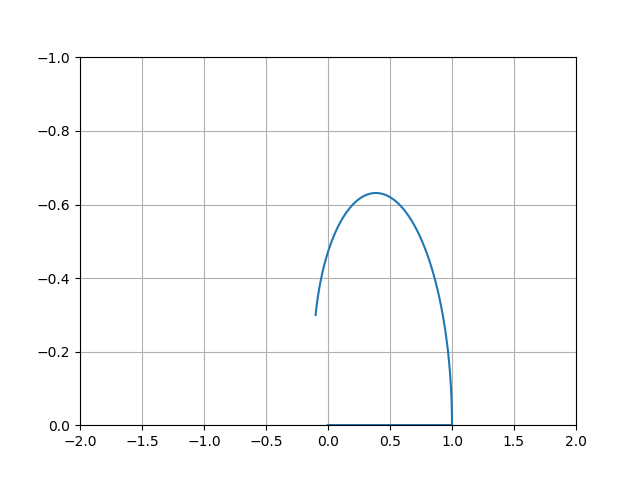
\includegraphics[width=0.7\linewidth]{Polarplot_A1(a).png}
    \caption{Different systems based on \zeta}
    \label{fig:Graph}
\end{figure}
\item
Verify the Polar Plot by running the following Code\\
\begin{lstlisting}
codes/ Ketan_A1(a).pyc
\end{lstlisting}
\end{enumerate}
